\chapter{Load Testing}
\label{ch:stresstesting}
Si è testata la capacità del sistema di offrire funzionalità senza interruzioni all'aumentare del carico. 
Si è optato per effettuare load test su backend tramite una suite di test JMeter. \cite{JMETER}

\section{Implementazione}

I test sono stati impostati per effettuare automaticamente la procedura di login per poi usare l'access token così ottenuto per autenticare le richieste inviate verso il backend.

Sono stati simulati 250 utenti concorrenti emettenti richieste a endpoint che prevedono l'uso di cache, ripetendo test con lifetime variabili delle entry in cache.
La dimensione della tabella di cache è stata mantenuta costante (60000 entry) generando casualmente valori di header \verb|AULOS-hash| (Ch. \ref{ch:caching}).
Il corpo delle richieste è stato fornito tramite un file .csv contenente tutte le possibili richieste generabili da un utente tramite la dashboard.

Testando la performance del backend quando sottoposto a un carico molto superiore a quello previsto dal caso d'uso dell'applicativo, è possibile avere un certo grado di sicurezza che il sistema sarà stabile una volta in utilizzo.



\section{Risultati}
Sono stati eseguiti test senza cache e con lifetime di entry in cache pari a 5, 15, 30 e 120 secondi. 
Una volta eseguiti tutti i test, si sono raccolte le seguenti statistiche, divise per durata delle entry di cache. Tutti i test hanno avuto la durata di un'ora.
L'hit ratio di entry in cache è stato calcolato secondo la seguente formula, dove x è il prodotto tra lifetime delle entry in cache e throughput finale (richieste/s) restituito da JMeter.
\begin{figure}[h!]

\begin{Large}




  \[
    f(x) = \left\{\begin{array}{lr}
        \frac{f(x-1)+\frac{cachesize - f(x-1)}{cachesize}}{cachesize}, & \text{ for } x\geq 1\\
        1 & \text{for } x=0
        \end{array}\right\} = \text{Cache hit ratio}
  \]
\caption{Cache hit ratio formula}
\label{fig:formula}
\end{Large}

\end{figure}

La figura~\ref{fig:throughput} rappresenta i dati relativi alle richieste al secondo mentre la figura~\ref{fig:hitratio} rappresenta la percentuale stimata di hit in cache durante il test, calcolata tramite la formula in fig.~\ref{fig:formula}.
\begin{figure}

\RawFloats
%\begin{subfloatrow}
\subfloat[Test throughput]{


\resizebox{7cm}{7cm}{%

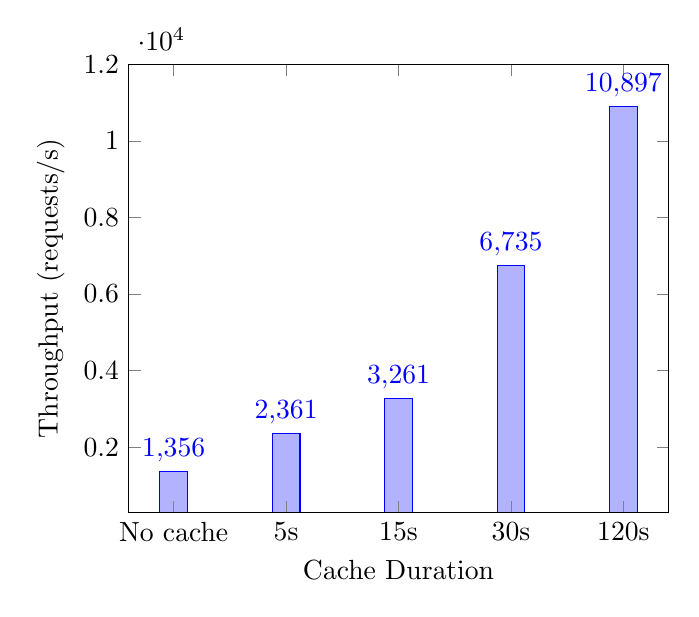
\begin{tikzpicture}

\begin{axis}[  
    hist/symbolic coords={No cache, 5s, 15s, 30s, 120s},
    area style,
    nodes near coords,
    ymax=12000,
    xlabel={Cache Duration},
    ylabel={Throughput (requests/s)}
    ]
\addplot+[ybar, mark=no] plot coordinates { (No cache, 1356) (5s, 2361) (15s, 3261) (30s, 6735) (120s, 10897) };
\end{axis}


\end{tikzpicture}
}
\label{fig:throughput}
}
\subfloat[Cache hit ratio]{

\resizebox{7cm}{7cm}
    ]
\addplot+[ybar, mark=no] plot coordinates { (No cache, 0) (5s, 17.86) (15s, 55.74) (30s, 96.55) (120s, 99.99) };
\end{axis}
\end{tikzpicture}
}
\label{fig:hitratio}
}
%\end{subfloatrow}
\caption{Dati estrapolati dai load test}

\end{figure}




